\documentclass[a4paper, 11pt, twoside]{article}
\usepackage{amssymb}
\usepackage{amsmath}
\usepackage{graphicx}
\graphicspath{ {images/} }
\begin{document}

\title{STAT6038 week 3 lecture 7 notes}
\author{Rui Qiu}
\date{2017-03-08}

\maketitle

The general linear model (multiple regression model)

\[
\begin{split}
	Y_i &=\beta_0+\beta_1X_{1i}+\beta_2X_{2i}+\cdots + \beta_k X_{ki} + \epsilon_i, i = 1, 2, \cdots, N\ \text{(population model}\\
	Y_i&=b_0+b_1x_{1i}+b_2x_{2i}+\cdots +b_kx_{ki}+e_i, i = 1,2,\cdots, n\ \text{sample model}
\end{split}
\]

In matrix notation:

\[
\begin{bmatrix}
	Y_1\\Y_2\\\vdots\\Y_n\\
\end{bmatrix}
=
\begin{bmatrix}
	1 & x_{11} & x_{21} & \cdots & x_{k1}\\
	1 & x_{12} & x_{22} & \cdots & x_{k2}\\
	\vdots & \vdots & \vdots & \ddots & \vdots\\
	1 & x_{1n} & x_{2n} & \cdots & x_{kn}\\
\end{bmatrix}
\begin{bmatrix}
	b_0\\b_1\\\vdots\\b_k\\
\end{bmatrix}
+
\begin{bmatrix}
	e_1\\e_2\\\vdots\\e_n\\
\end{bmatrix}
\]

\[
\begin{split}
	Y&=Xb+e \text{ estimated sample model}\\
	Y&=X\beta + \epsilon \text{ assumed population model}\\	
\end{split}
\]

For the special case of simple linear regression (where there is only 1 $X$ variable), the design matrix is just:

\[
X=
\begin{bmatrix}
	1 & x_1\\
	1 & x_2\\
	\vdots & \vdots\\
	1 & x_n\\
\end{bmatrix}
\text{ and }
\begin{bmatrix}
	Y_1\\Y_2\\\vdots\\Y_n\\
\end{bmatrix}
=
\begin{bmatrix}
	1 & x_1\\
	1 & x_2\\
	\vdots & \vdots\\
	1 & x_n\\
\end{bmatrix}
\begin{bmatrix}
	b_0\\b_1\\
\end{bmatrix}
+
\begin{bmatrix}
	e_1\\e_2\\\vdots\\e_n\\
\end{bmatrix}
=
\begin{bmatrix}
	b_0+b_1x_1\\
	b_0+b_1x_2\\
	\vdots\\
	b_0+b_1x_n\\
\end{bmatrix}
+
\begin{bmatrix}
	e_1\\e_2\\\vdots\\e_n\\
\end{bmatrix}
=
\begin{bmatrix}
	b_0+b_1x_1+e_1\\
	b_0+b_1x_2+e_2\\
	\vdots\\
	b_0+b_1x_n+e_n\\
\end{bmatrix}
\]

Similarly, in matrix notation, the least square estimates become 

\[\hat{\beta} = b = (X^TX)^{-1}(X^TY).\]

which holds for any number of $X$ variables.

For SLR:

\[
\begin{split}
	X^TX &=
\begin{bmatrix}
	1 & 1 & \cdots & 1\\
	x_1 & x_2 & \cdots & x_n\\
\end{bmatrix}
\begin{bmatrix}
	1 & x_1\\
	1 & x_2\\
	\vdots & \vdots \\
	1 & x_n\\
\end{bmatrix}
=\begin{bmatrix}
	n & \sum\limits^n_{i=1}x_i\\
	\sum\limits^n_{i=1}x_i & \sum\limits^n_{i=1}x_i^2\\
\end{bmatrix}\\
X^TY &=
\begin{bmatrix}
	1 & 1 & \cdots & 1\\
	x_1 & x_2 &\cdots & x_n\\
\end{bmatrix}
\begin{bmatrix}
	Y_1\\Y_2\vdots\\Y_n\\
\end{bmatrix}
=\begin{bmatrix}
	\sum\limits^n_{i=1}Y_i\\
	\sum\limits^n_{i=1}x_iY_i\\
\end{bmatrix}
\end{split}
\]

Finding the inverse of a $2\times 2$ matrix:

\[M=\begin{bmatrix}
	a & b\\c & d\\
\end{bmatrix}\implies
M^{-1}=\frac1{ad-bc}\begin{bmatrix}
	d & -b\\ -c & a\\
\end{bmatrix}
\]

So

\[(X^TX)^{-1}=\frac1{nS_{xx}}
\begin{bmatrix}
	\sum\limits^n_{i=1}x_i^2 & -\sum\limits^n_{i=1}x_i \\
	-\sum\limits^n_{i=1}x_i & n\\	
\end{bmatrix}
\]

Putting all those together:

\[\hat{\beta} = b = (X^TX)^{-1}(X^TY)=\frac1{nS_{xx}}
\begin{bmatrix}
		\sum\limits^n_{i=1}x_i^2 & -\sum\limits^n_{i=1}x_i \\
	-\sum\limits^n_{i=1}x_i & n\\	
\end{bmatrix}
\begin{bmatrix}
	\sum\limits^n_{i=1}Y_i\\
	\sum\limits^n_{i=1}x_iY_i\\
\end{bmatrix}
=\begin{bmatrix}
	\bar{Y}-\frac{S_{xy}}{S_{xx}}\bar{x}\\
	\frac{S_{xy}}{S_{xx}}\\
\end{bmatrix}
=\begin{bmatrix}
	b_0\\b_1\\
\end{bmatrix}
\]

A type of matrix that often has interesting properties is a variance-covariance matrix.

For example the vector of errors has variance-covariance matrix:

\[Var(\epsilon)=
\begin{bmatrix}
	Var(\epsilon_1) & Cov(\epsilon_1, \epsilon_2) & \cdots & Cov(\epsilon_1, \epsilon_N\\
	Cov(\epsilon_1, \epsilon_2) & Var(\epsilon_2) & \cdots &	 Cov(\epsilon_2, \epsilon_N\\
	\vdots & \vdots & \ddots & \vdots \\
	Cov(\epsilon_1, \epsilon_N) & Cov(\epsilon_2, \epsilon_N) & \cdots & Var(\epsilon_N)\\
\end{bmatrix}
\]

If two errors are independent of each other, covariance will be $0$, so the model-specific  assumptions that the errors are independent and have constant variance, can be summarized as:

\[Var(\epsilon)=\sigma^2I=\sigma^2
\begin{bmatrix}
	1 & 0 & \cdots & 0\\
	0 & 1 & \cdots & 0\\
	\vdots & \vdots & \ddots & \vdots\\
	0 & 0 & \cdots & 1\\	
\end{bmatrix}
=
\begin{bmatrix}
	\sigma^2 & 0 & \cdots & 0\\
	0 & \sigma^2 & \cdots & 0\\
	\vdots & \vdots & \ddots & \vdots\\
	0 & 0 & \cdots & \sigma^2\\	
\end{bmatrix}
\]

Similarly the variance-covariance matrix of the least square estimates can be shown to be:

\[Var(b)=\sigma^2(X^TX)^{-1}\]

For SLR, the diagonal elements of the matrix are:

\[
\begin{split}
	Var(b_0)&=\sigma^2\left(\frac{1}{n} + \frac{\bar{x}^2}{S_{xx}}\right)\\	
	Var(b_1)&=\frac{\sigma^2}{S_{xx}}\\
\end{split}
\]

We could take the square root of these variances to find standard errors for the least squares estimates of the coefficients, but first we will need to estimated the error variance.\\

Another matrix with interesting properties is the so-called hat matrix:

\[\hat{Y}=Xb=X(X^TX)^{-1}X^TY=HY, \text{ where } H=X(X^TX)^{-1}X^T.\]

The matrix $H$ is the hat matrix because when it multiplied by the observed $Y$ values, it produces the fitted values $\hat{Y}$. The hat matrix is an $n\times n$ matrix and the diagonal elements of this matrix are called the \textbf{leverage values:}

\[h_{ii} = \frac1{nS_{xx}}\sum\limits^n_{j=1}(x_j-x_i)^2.\\\]

There is one leverage value for each of the original $n$ observations and the leverage value can be used as a measure of how influential the corresponding observation was in the fitting of the  regression model.\\

Note that the vector of residuals (observed errors) can be written as:

\[e=Y-\hat{Y}=Y-HY=(1-H)Y\]

And the variance-covariance matrix of the residuals is:

\[Var(e)=\sigma^2(1-H)\]

which will be useful when we later standardize the residuals.\\

Finally we can also use the hat matrix to estimate the error variance (so we can find standard errors for the estimated coefficients). For SLR, where the error degrees of freedom are $n-2$:

\[\hat{\sigma}^2 = s^2 = \frac{SS_{Errors}}{n-2} = \frac{e^Te}{n-2} = \frac{(Y-\hat{Y})^T(Y-\hat{Y})}{n-2}=\frac{Y^T(1-H)Y}{n-2}.\]

\paragraph{Leverage (Influence)}

http://data.library.virginia.edu/diagnostic-plots/

This plot helps us to find influential cases (i.e., subjects) if any. Not all outliers are influential in linear regression analysis (whatever outliers mean). Even though data have extreme values, they might not be influential to determine a regression line. That means, the results wouldn’t be much different if we either include or exclude them from analysis. They follow the trend in the majority of cases and they don’t really matter; they are not influential. On the other hand, some cases could be very influential even if they look to be within a reasonable range of the values. They could be extreme cases against a regression line and can alter the results if we exclude them from analysis. Another way to put it is that they don’t get along with the trend in the majority of the cases.

Unlike the other plots, this time patterns are not relevant. We watch out for outlying values at the upper right corner or at the lower right corner. Those spots are the places where cases can be influential against a regression line. Look for cases outside of a dashed line, Cook’s distance. When cases are outside of the Cook’s distance (meaning they have high Cook’s distance scores), the cases are influential to the regression results. The regression results will be altered if we exclude those cases.

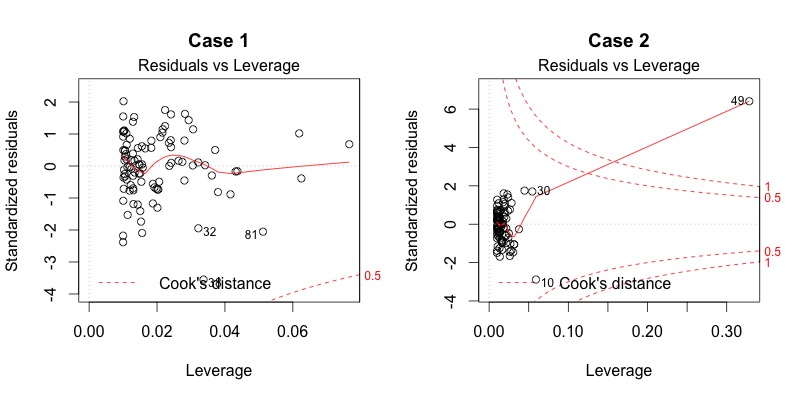
\includegraphics[width=\textwidth]{leverage.jpeg}

Case 1 is the typical look when there is no influential case, or cases. You can barely see Cook’s distance lines (a red dashed line) because all cases are well inside of the Cook’s distance lines. In Case 2, a case is far beyond the Cook’s distance lines (the other residuals appear clustered on the left because the second plot is scaled to show larger area than the first plot). The plot identified the influential observation as 49th. If I exclude the 49th case from the analysis, the slope coefficient changes from 2.14 to 2.68 and $R^2$ from .757 to .851. Pretty big impact!\\

A point of large leverage (high influence) is one that has an $x$ value that is a long way from $\bar{x}$ (i.e. it is remote from the bulk of the data -- outlying in the $x$ direction) $\implies$ $h_{ii}$ will be large, close to $1$.\\

Note, in general, $\sum^n_{i=1}h_{ii} = p$, where $p$ is the number of mean parameters in the model.\\

For SLR, $p=2$ which are $\hat{\beta_0}, \hat{\beta_1}$\\

Large leverage is not always a problem, some comparison is needed. It is ok that large leverage point on the regression line, but not ok it is not on it!\\

Note: Large leverage is often defined as $> 2\cdot \frac{\sum h_{ii}}{n}$ i.e. more than twice average leverage!

\end{document}